%=============================================================================
%  MindGuard -- Springer LNNS version, prepared for ICIDA 2026
%  (5th Intl. Conference on Innovations in Data Analytics, Kolkata, Dec 2026)
%
%  COMPILE:  pdflatex mindguard_springer   (twice, for cross-references)
%  No BibTeX pass needed -- references are embedded in thebibliography.
%
%  Requires llncs.cls, which Overleaf provides. If compiling locally and it is
%  missing, fetch the Springer LNCS/LNNS author kit.
%
%  >>> BEFORE SUBMITTING <<<
%  1. Confirm the institute/department line below is correct for all authors.
%  2. Verify EVERY reference against the real publication (vol/no/pages/DOI).
%  3. ICIDA requires a MINIMUM of 10 pages. There is no stated maximum.
%  4. Do NOT add accuracy/precision/recall numbers unless you measure them.
%=============================================================================

\documentclass[runningheads]{llncs}

\usepackage{amsmath,amssymb,amsfonts}
\usepackage{algorithmic}
\usepackage{graphicx}
\usepackage{booktabs}
\usepackage{xcolor}
\usepackage[hidelinks]{hyperref}
\usepackage{url}

\begin{document}

\title{MindGuard: A Privacy-Preserving Multimodal Mental Wellness
Companion with Fully On-Device Neural Speech Synthesis}

\titlerunning{MindGuard: Privacy-Preserving Multimodal Mental Wellness}

\author{%
Bibijan H Rajpal\inst{1} \and
Shravani\inst{1} \and
Tejaswini N\inst{1}}

\authorrunning{B. H. Rajpal et al.}

\institute{Department of Computer Science and Engineering,\\
B.N.M. Institute of Technology, Bengaluru, India\\
\email{bibijanrajpal@gmail.com}\\
\email{shravanichalla01@gmail.com}\\
\email{tejaswinintejaswinin9@gmail.com}}

\maketitle

\begin{abstract}
Conversational mental-wellness applications typically transmit the user's text,
voice, and facial imagery to third-party cloud inference services, creating a
privacy exposure difficult to reconcile with the sensitivity of the domain.
This paper presents MindGuard, a multimodal wellness companion built around an
inversion of that default: all speech synthesis and visual affect estimation
execute entirely within the user's browser, and no audio or video frame is
transmitted at any point. An 82M-parameter neural text-to-speech model runs
client-side through ONNX Runtime Web with a WebGPU-to-WebAssembly fallback.
Emotion inference uses deliberately non-learned estimators, a weighted lexicon
classifier for text and a hand-crafted optical heuristic for video, trading
measured accuracy for decision traceability and a zero-byte model download. A
triple-weighted moving average aggregates per-entry emotion into a burnout
index, propagating recency, confidence, and modality reliability as
multiplicative weights so that low-trust evidence is attenuated rather than
discarded. A crisis-safety path is architecturally exempt from every
personalisation layer, enforced by regression tests. We additionally report a
negative result: an earlier revision derived voice and video emotion from a
CRC32 checksum of the uploaded media, producing deterministic but meaningless
labels that silently contaminated the burnout index. We state explicitly that
no accuracy evaluation is reported; no estimator has been benchmarked against a
labelled corpus, and no precision, recall, or F1 figure is claimed. The
contribution is architectural, validated by 65 passing regression tests, and a
pre-specified evaluation protocol is given for subsequent work.

\keywords{Mental health informatics \and On-device inference \and Privacy-preserving machine learning \and Neural text-to-speech \and Multimodal fusion \and Affective computing \and Explainable systems \and WebAssembly}
\end{abstract}

\section{Introduction}
\label{sec:intro}
%=============================================================================

Self-reported psychological distress among students and early-career
professionals has motivated a large class of conversational wellness
applications. The dominant implementation pattern routes user input to a
hosted large language model and hosted speech and vision services. This
pattern is operationally convenient but has a structural consequence: the
most sensitive utterances a user will ever produce, together with their
facial imagery and voice, leave the device.

MindGuard was built to test whether a useful multimodal wellness companion
can be constructed while holding two constraints:

\begin{enumerate}
\item \textbf{No audio or video leaves the device.} Speech synthesis and
visual affect estimation execute locally, in the browser.
\item \textbf{Every inference is traceable.} A user-visible emotional
judgement must be attributable to a specific, inspectable cause.
\end{enumerate}

These constraints are costly, and this paper does not present them as free.
Constraint~2 in particular led us to reject pretrained affect classifiers in
favour of non-learned estimators, which means we cannot report competitive
accuracy figures --- and, as Section~\ref{sec:noeval} states plainly, we do not
report any. What we offer instead is a complete, reproducible architecture in
which the cost of each privacy decision is made explicit.

\subsection{Contributions}

\begin{itemize}
\item A working architecture for browser-resident neural speech synthesis in a
mental-health context, including the execution-provider fallback path
(Section~\ref{sec:tts}).
\item A confidence-propagating burnout aggregation function whose weights are
multiplicative across three independent trust dimensions
(Section~\ref{sec:burnout}).
\item A safety-first control-flow pattern in which crisis handling bypasses all
personalisation layers, enforced by regression tests
(Section~\ref{sec:safety}).
\item A documented negative result: the detection and removal of
checksum-derived pseudo-inference, and the substitution of explicit
uncertainty (Section~\ref{sec:negative}). We argue this failure mode is
under-reported and easy to reproduce accidentally.
\item An explicit non-evaluation statement and a pre-registered evaluation
protocol (Sections~\ref{sec:noeval} and \ref{sec:protocol}).
\end{itemize}

%=============================================================================
\section{Related Work}
%=============================================================================

\subsection{Conversational Agents for Mental Wellness}
Rule-based and hybrid conversational agents have been evaluated in controlled
trials; Fitzpatrick et al. reported a randomised trial of a cognitive
behavioural therapy chatbot \cite{woebot}, and Inkster et al. examined an
empathy-driven agent in a real-world cohort \cite{wysa}. Both deployments
depend on server-side inference. Our work differs not in conversational
ambition --- which is smaller --- but in placing the speech and vision layers
on the client.

\subsection{Lexicon-Based Affect Estimation}
Weighted-lexicon sentiment analysis has a long precedent. LIWC established
dictionary-based psychological text measurement \cite{liwc}, and VADER
demonstrated that a hand-tuned, rule-augmented lexicon with intensity
modifiers remains competitive with learned models on short social text
\cite{vader}. Our text classifier is architecturally of this family: it extends
a weighted lexicon with multiplicative intensity modulation and margin-derived
confidence. Unlike VADER, which was validated against human-annotated
corpora, ours is unvalidated --- a deficiency we state rather than obscure.

\subsection{Facial Expression Recognition}
Learned facial expression recognition is conventionally trained on corpora such
as FER-2013 \cite{fer2013} or AffectNet \cite{affectnet}, and modern systems
achieve substantially better accuracy than any heuristic. We deliberately do
not compete on that axis. Our visual component is a hand-crafted optical
heuristic chosen for a different objective function: zero model download, no
frame transmission, and per-decision traceability. Section~\ref{sec:vision}
reports its failure modes candidly.

\subsection{On-Device Neural Inference}
The maturation of ONNX Runtime Web \cite{onnxweb} and the WebGPU API
\cite{webgpu} has made browser-resident execution of small neural models
practical. We apply this to speech synthesis using a compact open neural TTS
model \cite{kokoro}. To our knowledge, the combination of fully client-side
neural TTS with an explicitly privacy-motivated mental-health use case is not
well represented in the applied literature.

\subsection{Burnout Measurement}
Clinical burnout instruments such as the Maslach Burnout Inventory
\cite{maslach} and depression screeners such as PHQ-9 \cite{phq9} are
administered as validated questionnaires. Our burnout index is explicitly
\emph{not} a clinical instrument and is not calibrated against one; it is a
longitudinal engagement signal derived from passive interaction history. We
regard conflation of the two as a significant risk in this application
category and address it in Section~\ref{sec:limits}.

%=============================================================================
\section{System Architecture}
%=============================================================================

MindGuard is a three-tier system, shown in Fig.~\ref{fig:arch}.

\textbf{Client tier.} A React~19 single-page application built with Vite,
containing the visual affect estimator, the neural TTS engine, the multimodal
fusion stage, and a procedural ambient audio synthesiser. A React
Native/Expo client shares the API contract.

\textbf{Service tier.} A Django~4.2 application exposing a Django REST
Framework API of 20 endpoints, served by Gunicorn. This tier owns the text
classifier, the burnout aggregator, authentication, and the safety layer.

\textbf{Data tier.} PostgreSQL~16 in production via \texttt{psycopg}~3;
SQLite in development. Engine selection is governed by a single
\texttt{DATABASE\_URL} environment variable parsed by
\texttt{dj-database-url}, so that schema and query code are identical across
both.

\begin{figure}[htbp]
\centering
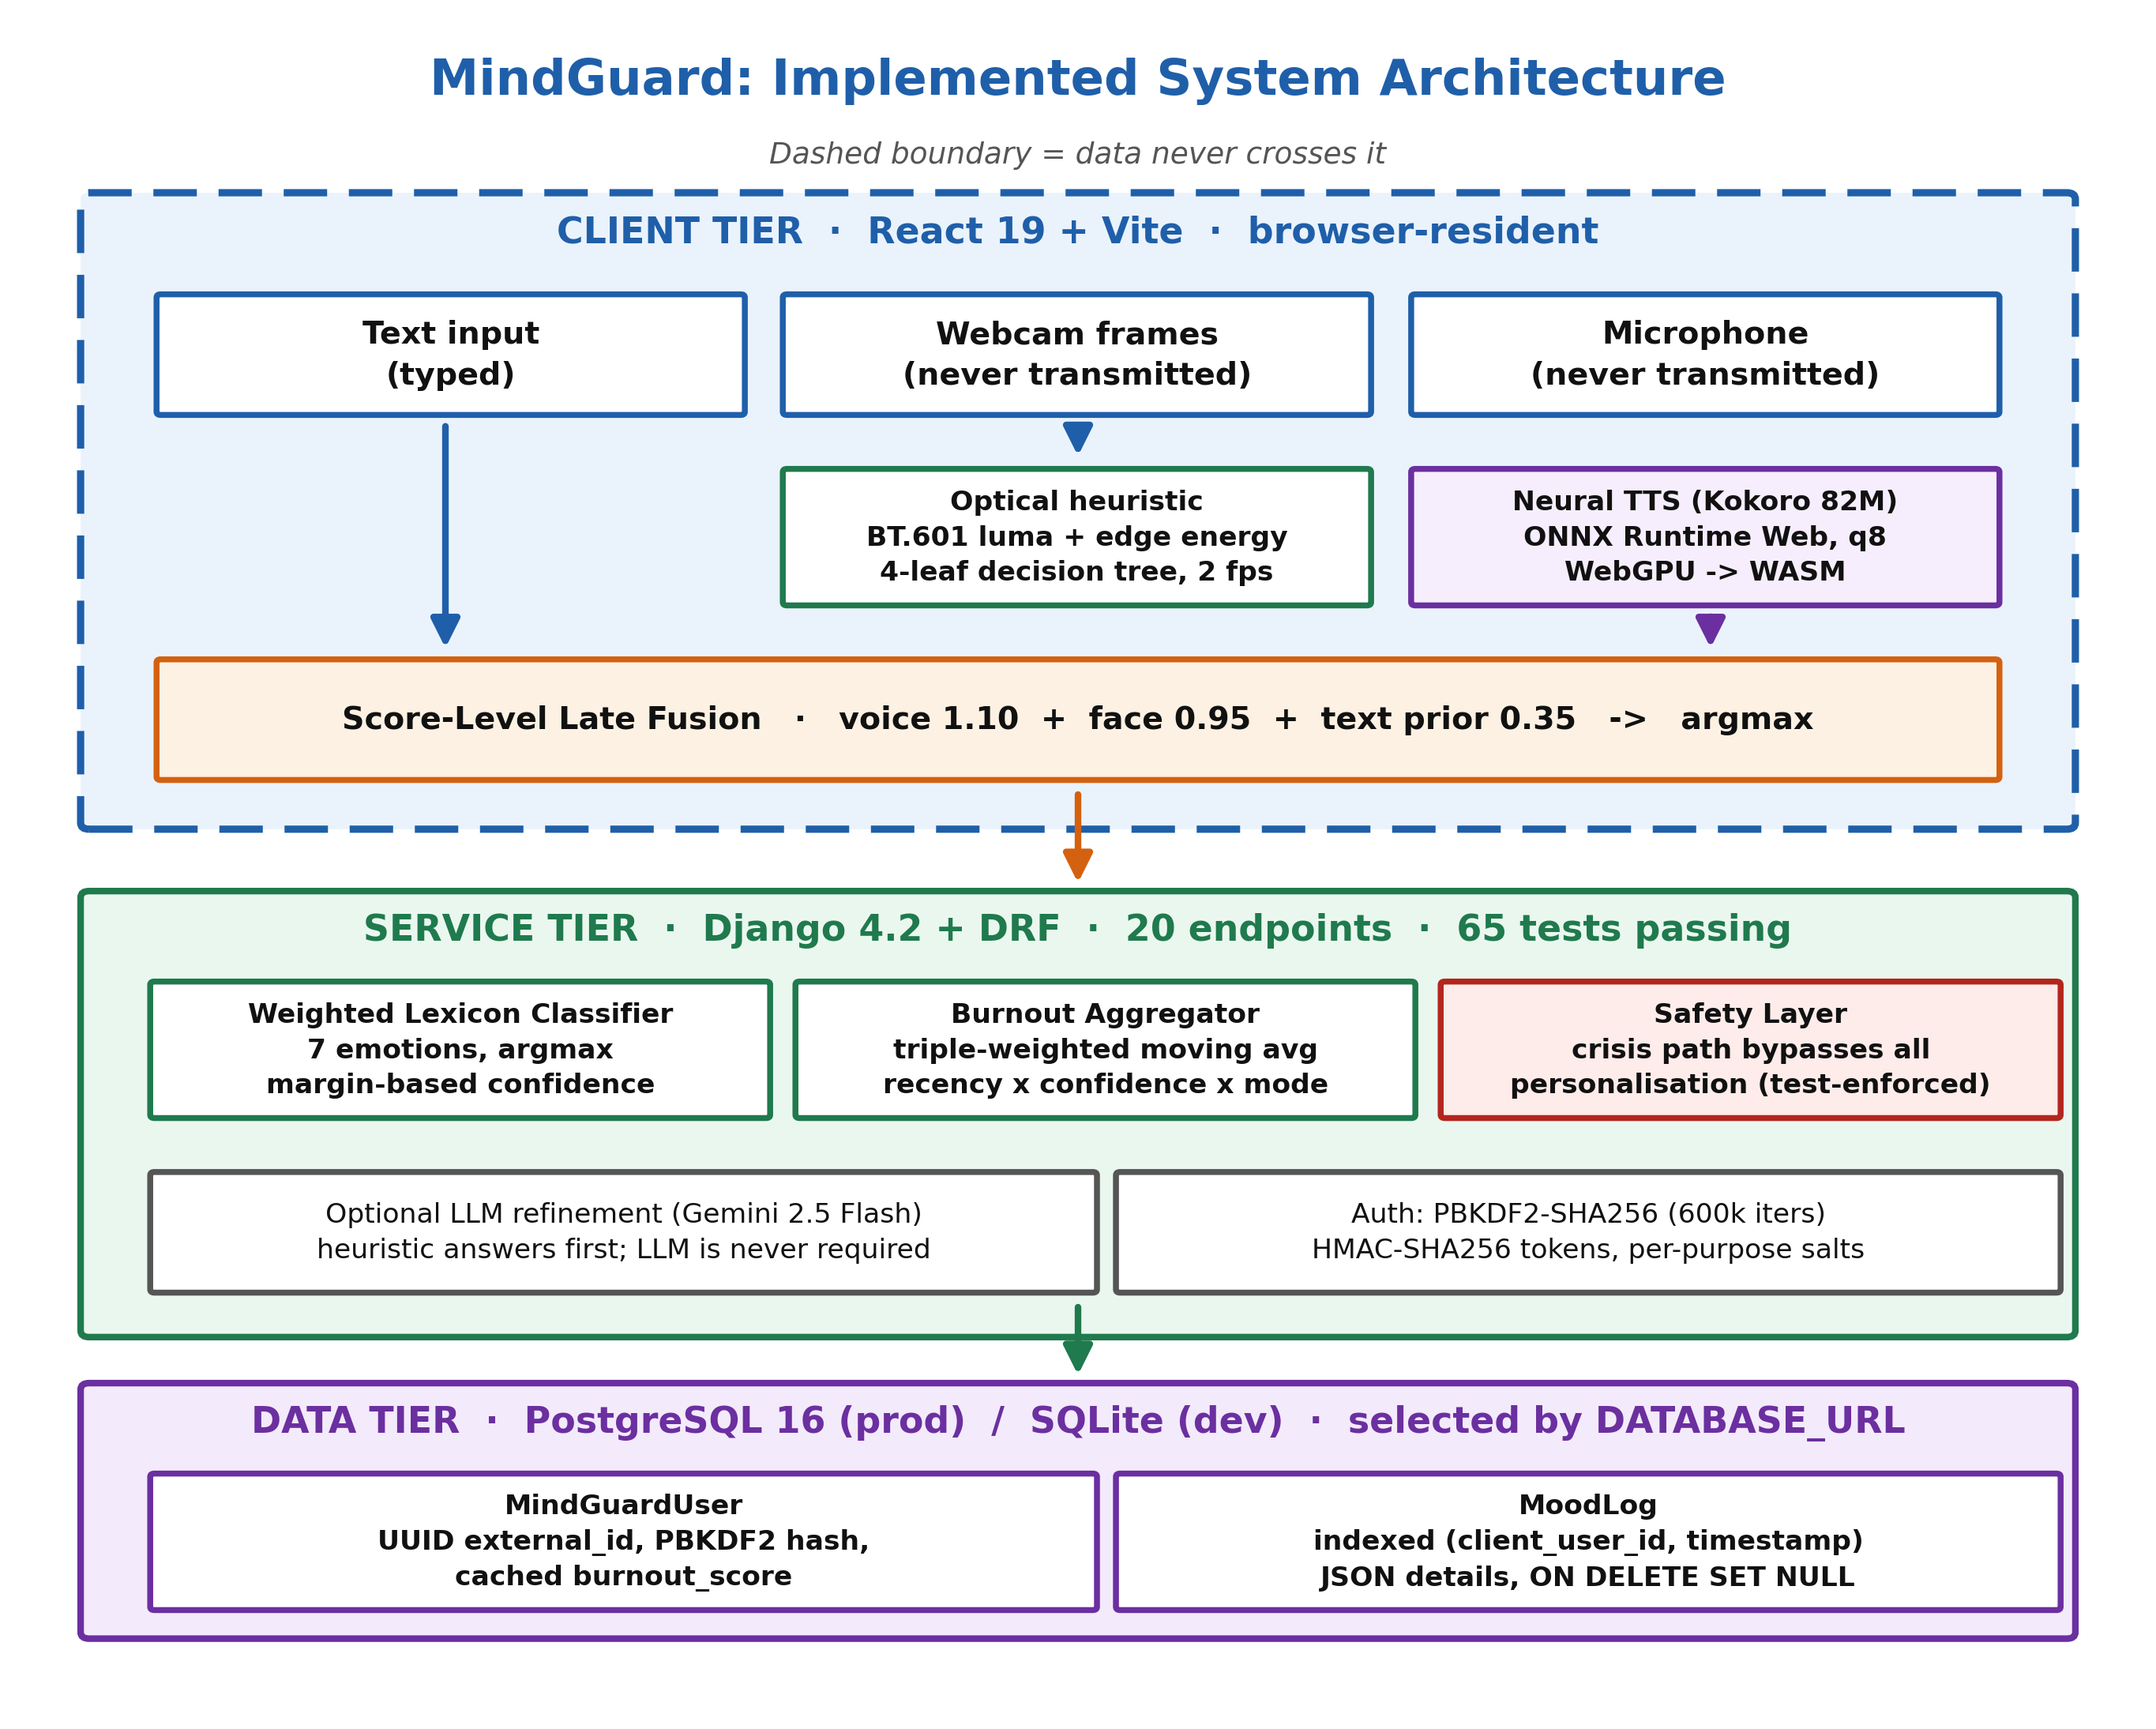
\includegraphics[width=\textwidth]{fig1_architecture.png}
\caption{Implemented three-tier architecture. The dashed boundary encloses the
client tier; webcam frames and microphone audio are processed within it and are
never transmitted. Note that no component of the affect pipeline contains
trained parameters.}
\label{fig:arch}
\end{figure}

A deliberate asymmetry governs tier placement: \emph{modalities whose raw form
is irreducibly identifying} --- audio and video --- are processed only on the
client, whereas text, which the user has already chosen to commit to words,
is processed server-side where the lexicon and aggregation logic can be
centrally versioned and tested.

%=============================================================================
\section{Text Emotion Classification}
%=============================================================================

\subsection{Weighted Lexicon Scoring}
Let $x$ be the normalised input utterance and $E$ the label set
$\{$\textit{happy}, \textit{calm}, \textit{neutral}, \textit{sad},
\textit{fatigued}, \textit{anxious}, \textit{stressed}$\}$, $|E| = 7$. Each
$e \in E$ has an associated term set $T_e$ in which every term $t$ carries a
hand-assigned weight $w_t$. The raw score for emotion $e$ is

\begin{equation}
s_e = \mu(x) \sum_{t \in T_e} w_t \cdot \mathbb{I}[t \in x]
\end{equation}

where $\mathbb{I}$ is the indicator function. Weights encode clinical salience
rather than frequency; for example the term \textit{burnout} carries
$w_t = 3.2$, dominating a general term such as \textit{tired}.

\subsection{Multiplicative Intensity Modulation}
Rather than enumerating separate lexicon entries for modified phrases, a single
multiplier is applied:

\begin{equation}
\mu(x) = 1.0 + 0.10\,n_{\text{int}}(x) - 0.08\,n_{\text{soft}}(x)
\end{equation}

with $n_{\text{int}}$ and $n_{\text{soft}}$ the counts of intensifiers
(\textit{very}, \textit{extremely}) and softeners (\textit{slightly},
\textit{a bit}). The asymmetry ($0.10$ versus $0.08$) reflects a conservative
bias: amplification is trusted marginally more than hedging, since users
frequently minimise distress.

\subsection{Margin-Derived Confidence}
The predicted label is $\hat{e} = \arg\max_{e \in E} s_e$. Let $s_{(1)}$ and
$s_{(2)}$ be the largest and second-largest scores. Confidence is

\begin{equation}
c = \mathrm{clamp}\!\left(0.58 + \frac{s_{(1)} - s_{(2)}}{6},\; 0.58,\; 0.97\right)
\label{eq:conf}
\end{equation}

Confidence is thus a function of \emph{separation}, not magnitude: two
near-tied candidates yield low confidence even when both score highly. The
upper clamp at $0.97$ encodes that a lexicon is never certain; the lower clamp
at $0.58$ prevents a near-tie from collapsing the entry's weight to zero in
the downstream aggregation (Section~\ref{sec:burnout}).

\subsection{Hybrid Rule-LLM Cascade}
A hosted LLM (Gemini 2.5 Flash) optionally refines the response wording.
Crucially, the ordering is heuristic-first: the lexicon classifier always
produces a complete result, the LLM revises presentation, and the two are
merged. If the API key is absent, rate-limited, or the service is unavailable,
the heuristic result \emph{is} the response. The system therefore has no hard
runtime dependency on a third-party model. The API key is held server-side and
is never exposed to the client.

%=============================================================================
\section{Visual Affect Estimation}
\label{sec:vision}
%=============================================================================

The visual component is a two-stage estimator: hand-crafted optical feature
extraction followed by a priority-ordered rule-based decision tree. It contains
no trained parameters.

\subsection{Feature Extraction}
Each sampled frame is drawn to an offscreen canvas downscaled to
$160 \times 120$ px. Per-pixel luminance uses the ITU-R BT.601 luma transform
\cite{bt601}:

\begin{equation}
Y = 0.299R + 0.587G + 0.114B
\end{equation}

Three regional means are accumulated over the central crop
($x \in [0.25w, 0.75w]$, $y \in [0.20h, 0.85h]$): the global face-region mean
$\bar{Y}$, a brow-band mean $\bar{Y}_b$ over $y \in [0.28h, 0.42h]$, and a
mouth-band mean $\bar{Y}_m$ over $y \in [0.62h, 0.78h]$. Edge energy is the
normalised first-order horizontal finite difference:

\begin{equation}
\mathcal{E} = \frac{1}{|R|}\sum_{(x,y) \in R} \bigl| Y(x,y) - Y(x{+}1,y) \bigr|
\end{equation}

Brow furrowing produces near-vertical shadow creases, to which a horizontal
gradient is maximally responsive. Two scale-normalised contrast ratios are
then formed:

\begin{equation}
\rho_b = \frac{\bar{Y}_b}{\bar{Y} + 1}, \qquad
\rho_m = \frac{\bar{Y}_m}{\bar{Y} + 1}
\end{equation}

Ratios rather than absolute luminances are used so that the features are
partially invariant to ambient illumination. The denominator is the mid-face
mean excluding both bands rather than the global mean, for the reason given in
Section~\ref{sec:vision}; see (\ref{eq:decoupled}).

\subsection{Rule-Based Classification}
Classification is a four-leaf decision tree, evaluated in priority order:

\begin{algorithmic}[1]
\IF{$\rho_b < 0.88$ \OR $\mathcal{E} > 18$}
    \STATE \textbf{return} \textit{stressed}
\ELSIF{$\rho_m > 1.08$ \AND $\rho_b \geq 0.95$}
    \STATE \textbf{return} \textit{happy}
\ELSIF{$\bar{Y} < 75$ \OR $\mathcal{E} < 6$}
    \STATE \textbf{return} \textit{fatigued}
\ELSE
    \STATE \textbf{return} \textit{calm}
\ENDIF
\end{algorithmic}

Tension is reported as
$\tau = \min\bigl(92,\, 55 + 100(1 - \rho_b)\bigr)$.
The evaluation order is not arbitrary: \textit{stressed} is tested first
because, in a wellness context, the cost of a missed distress signal exceeds
the cost of a false positive.

\subsection{Sampling Rate}
Analysis is throttled to one frame every 500\,ms (2\,fps). The pixel loop is
synchronous JavaScript; at native frame rate it saturates a core and stalls UI
paint. The throttle is also substantively defensible --- affective state does
not vary meaningfully on a sub-second scale.

\subsection{Acknowledged Failure Modes}
We report three limitations of this estimator directly, as they bound any
interpretation of its output.

\textbf{No face detection.} The pipeline performs no face-presence check;
regions are fixed fractions of the frame and a centred, front-facing subject
is assumed. A frame containing no face still yields a label. Gating the
classifier behind a lightweight detector is the appropriate remedy.

\textbf{Threshold-margin confidence (revised).} An earlier revision returned
constant confidence values in $[0.89, 0.96]$ per branch. These were trust
priors over rules rather than estimated quantities, and reporting them as
confidence overstated the certainty of a parameter-free heuristic. We replaced
them with a margin-derived construction analogous to (\ref{eq:conf}). For the
selected branch we compute a normalised decisiveness $d \in [0,1]$ --- the
maximum normalised margin across disjunctive predicates, the minimum across
conjunctive ones, and for the fall-through \textit{calm} leaf the distance to
the nearest boundary not crossed --- and map it linearly onto a deliberately
bounded interval:

\begin{equation}
c_{\text{vis}} = 0.55 + 0.35\,d
\label{eq:visconf}
\end{equation}

The ceiling of $0.90$ is intentional: no configuration of a hand-tuned
heuristic should report near-certainty. Empirically the resulting curve
behaves as intended --- sweeping brow luminance across the decision boundary
produces confidences of $0.77$, $0.71$, $0.59$ for \textit{calm} as the
boundary is approached, $0.65$ and $0.83$ for \textit{stressed} just past it,
saturating at $0.90$ only once the margin exceeds the normaliser.

\textbf{Low-signal rejection.} Because the estimator performs no face
detection, we added an explicit structural-signal test. Below an edge-density
floor the frame contains no discernible facial structure --- a blank wall, an
obstructed lens, or severe underexposure all qualify --- and confidence is
capped at $0.30$ with a \texttt{lowSignal} flag, regardless of which branch
the thresholds selected. Without this test a featureless frame was returned as
\textit{fatigued} at $0.90$ confidence, the maximum the system can express,
for an input containing no face at all. This applies the same principle as the
\texttt{unscored} outcome of Section~\ref{sec:negative}: absence of signal is
reported as absence of knowledge rather than resolved into a label.

\textbf{Illumination coupling.} The predicate $\bar{Y} < 75 \Rightarrow$
\textit{fatigued} conflates a dimly lit room with a fatigued subject. A
per-session luminance baseline captured at calibration, with thresholds
expressed relative to it, would decouple the two.

\textbf{Inter-region coupling (corrected).} Normalising every regional ratio
by the same global mean $\bar{Y}$ coupled the ratios to one another, because
$\bar{Y}$ contains both bands. Sweeping mouth luminance exposed the
consequence: the \textit{happy} leaf fired only within a narrow band, and as
the mouth region brightened further $\bar{Y}$ rose, $\rho_b$ fell below the
conjunctive gate $\rho_b \geq 0.95$, and classification reverted to
\textit{calm}. A broad smile --- the strongest available positive signal ---
was therefore undetectable, with measured outputs of \textit{happy} at mouth
luminance $155$ but \textit{calm} at $170$ and $190$.

The defect was structural rather than a threshold miscalibration, so we
replaced the reference with a mid-face mean $\bar{Y}_n$ computed over the crop
\emph{excluding} both bands:

\begin{equation}
\rho_b = \frac{\bar{Y}_b}{\bar{Y}_n + 1}, \qquad
\rho_m = \frac{\bar{Y}_m}{\bar{Y}_n + 1}
\label{eq:decoupled}
\end{equation}

Since $\bar{Y}_n$ is independent of both band luminances, each ratio is now
independent of the other region. The response became monotone as intended ---
\textit{happy} at confidence $0.61$, $0.82$, $0.90$ for increasing mouth
luminance. A uniform frame still yields $\rho = 1$ under
(\ref{eq:decoupled}), so the thresholds retain their calibration relative to
unity; the brow test is now marginally more sensitive, as the dark band no
longer depresses its own denominator.

%=============================================================================
\section{Multimodal Late Fusion}
%=============================================================================

Modalities are classified independently and combined at score level, as
shown in Fig.~\ref{fig:pipeline}. Each
modality $k$ contributes its score vector scaled by a fixed reliability
coefficient $\lambda_k$ --- voice $1.10$, face $0.95$, and text prior $0.35$:

\begin{equation}
S_e = \sum_{k \in K} \lambda_k \, s_e^{(k)}, \qquad
\hat{e} = \arg\max_{e \in E} S_e
\end{equation}

\begin{figure}[htbp]
\centering
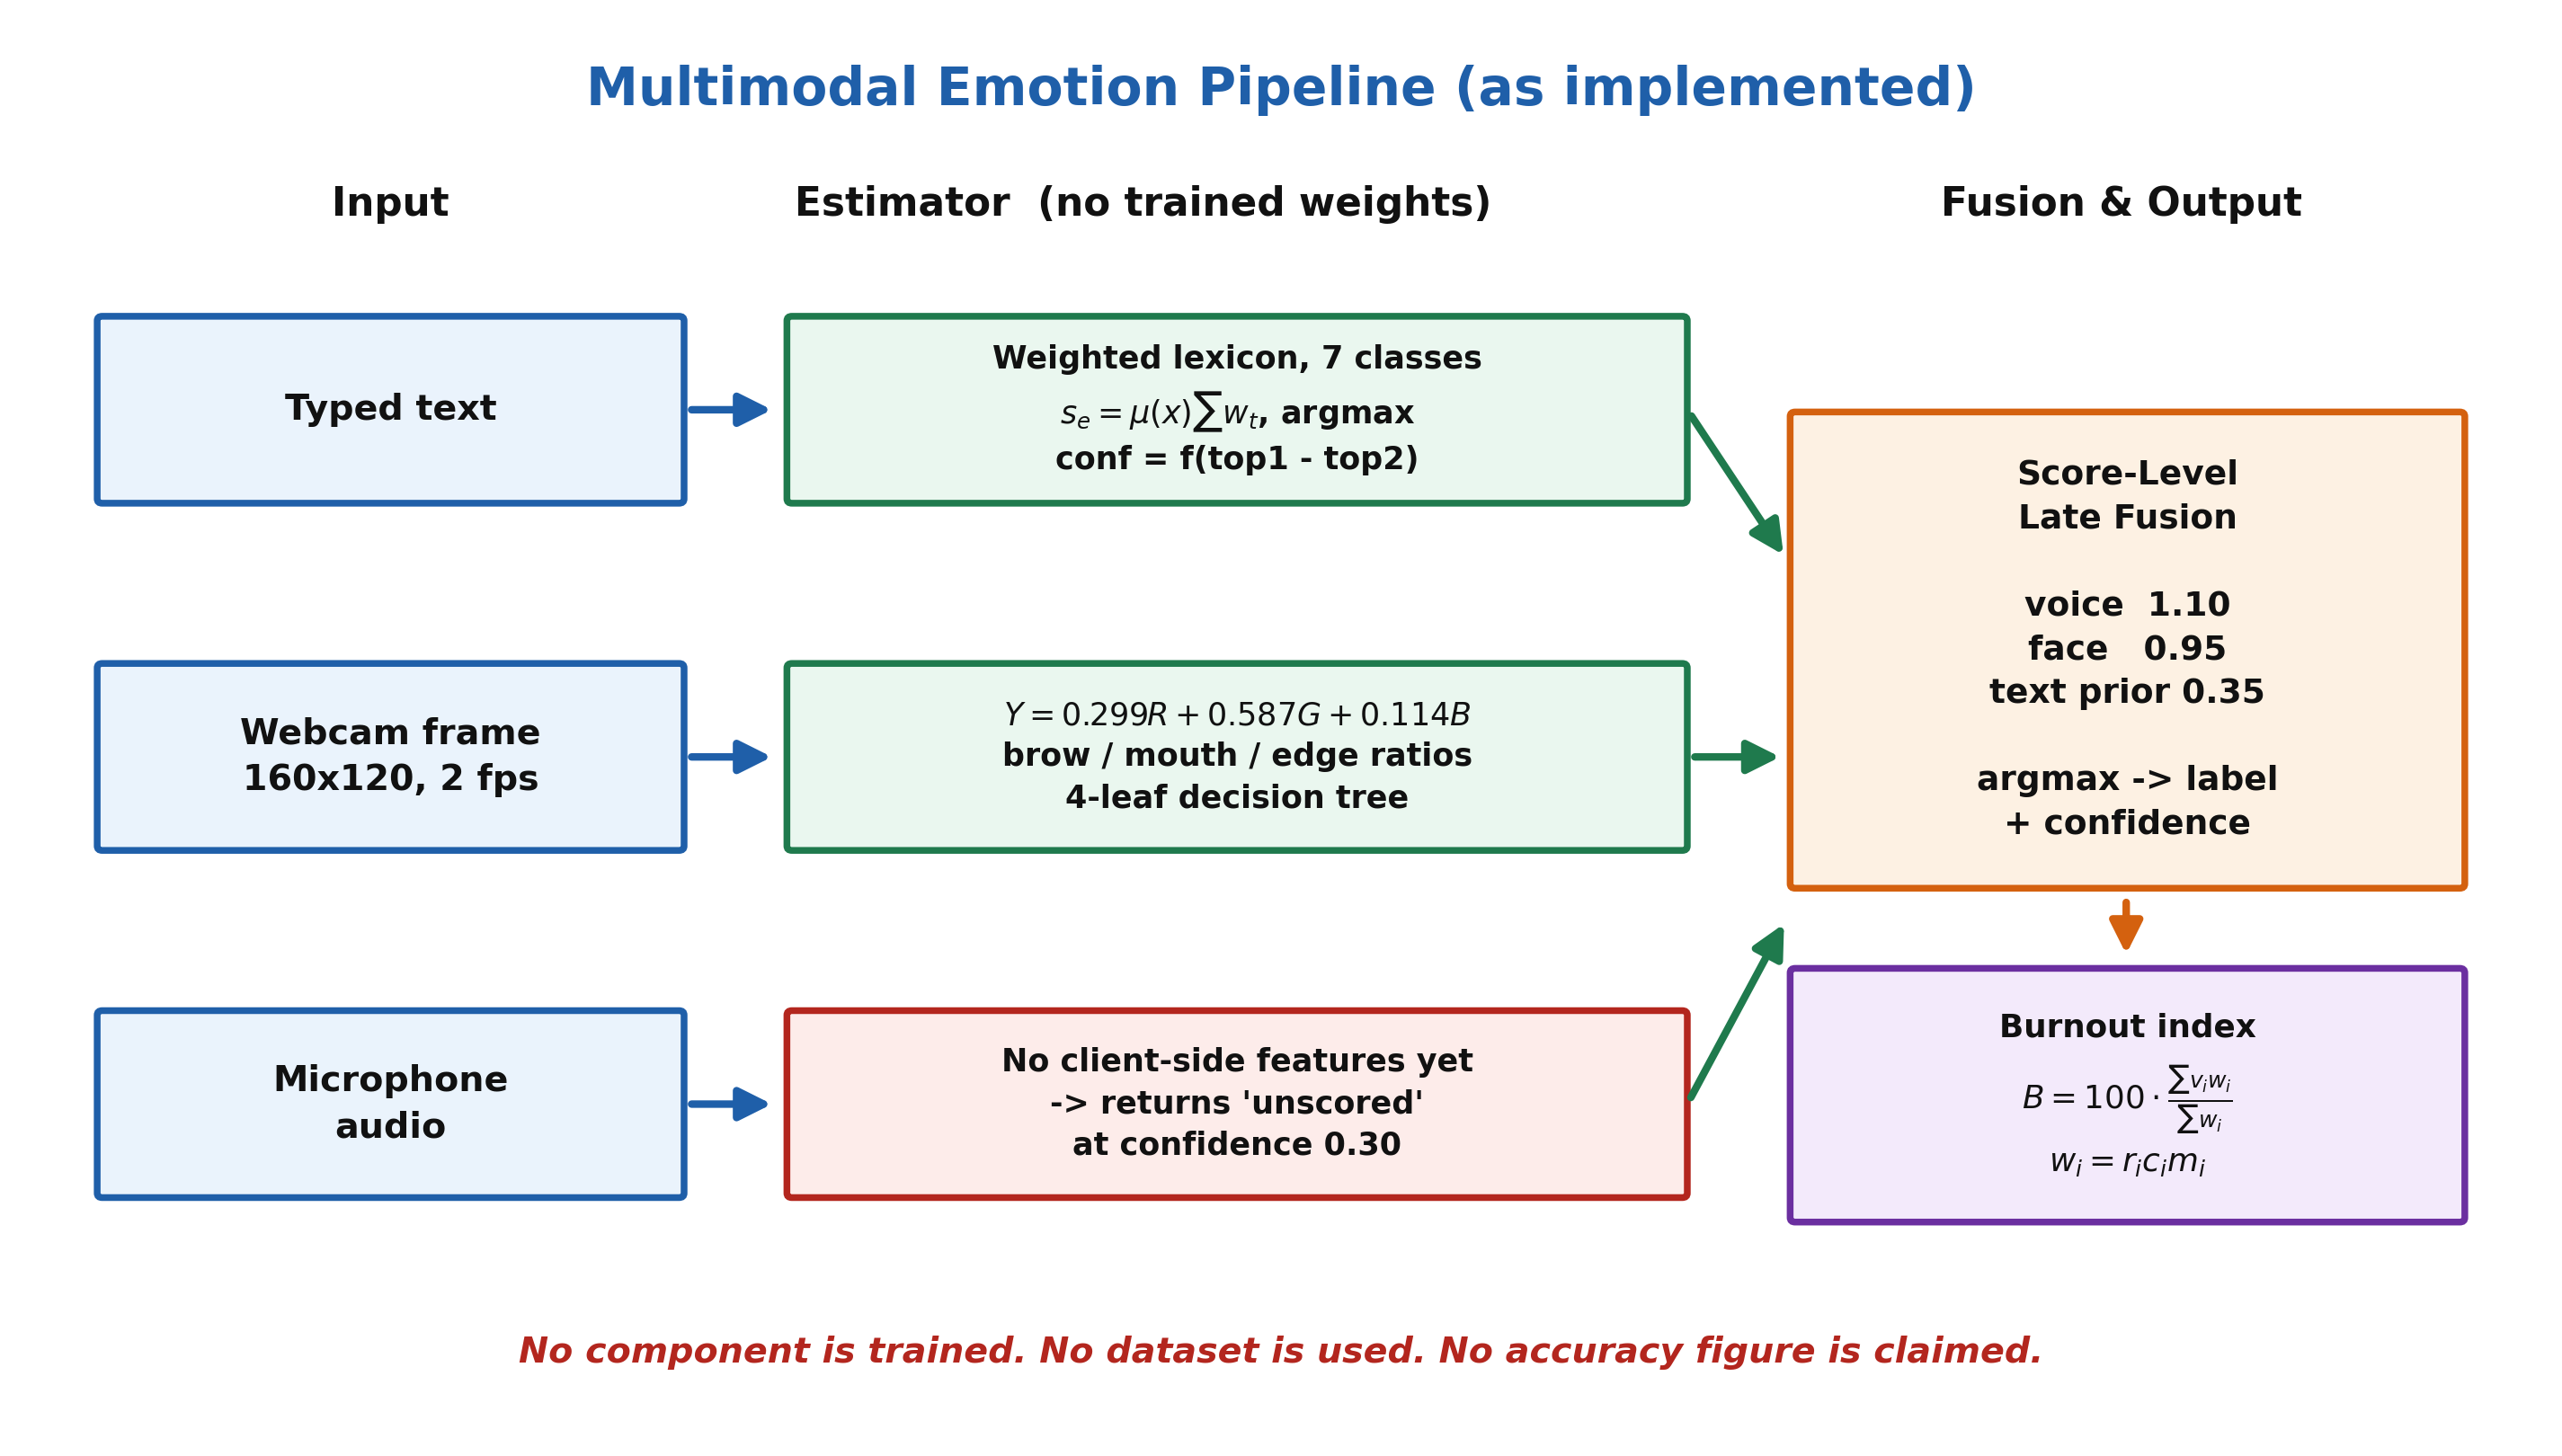
\includegraphics[width=\textwidth]{fig2_pipeline.png}
\caption{Multimodal emotion pipeline as implemented. Each modality is
classified independently and combined at score level, so the system degrades
gracefully when a modality is unavailable. The voice path currently returns
\texttt{unscored} because client-side acoustic features are not yet computed
(Section~\ref{sec:negative}).}
\label{fig:pipeline}
\end{figure}

Late fusion is chosen over early (feature-level) fusion for a specific
operational reason: it degrades gracefully. A user may decline camera
permission, be in a noisy environment, or type only. Early fusion over a
concatenated feature vector requires all modalities to be present; late fusion
over score vectors requires only one. Displayed meters are smoothed by an
exponential moving average, $v_t = 0.6\,v_{t-1} + 0.4\,v_t^{\text{raw}}$
($\alpha = 0.4$), to suppress per-frame jitter.

%=============================================================================
\section{Burnout Quantification}
\label{sec:burnout}
%=============================================================================

\subsection{Emotion-to-Burden Mapping}
Each label maps to a scalar burden value $v_e \in [0,1]$:
\textit{calm} $0.12$, \textit{happy} $0.18$, \textit{neutral} $0.42$,
\textit{sad} $0.58$, \textit{fatigued} $0.66$, \textit{anxious} $0.78$,
\textit{stressed} $0.90$. Unrecognised labels default to $0.42$.

\subsection{Triple-Weighted Moving Average}
Over the $n = 10$ most recent entries, indexed $i = 0$ (newest) to $n-1$,
three independent weights are formed. Recency decays hyperbolically:

\begin{equation}
r_i = \frac{1}{1 + 0.38\,i}
\end{equation}

Confidence is floored, and modality reliability $m$ is drawn from
$\{$combo $1.15$, voice $1.05$, text $1.00$, video $0.95\}$:

\begin{equation}
w_i = r_i \cdot \max(c_i, 0.45) \cdot m_i
\label{eq:weight}
\end{equation}

The burnout index is the weighted mean scaled to a 0--100 range:

\begin{equation}
B = 100 \cdot \frac{\sum_{i=0}^{n-1} v_i\, w_i}{\sum_{i=0}^{n-1} w_i}
\end{equation}

and is banded as \textit{High} ($B \geq 70$), \textit{Moderate}
($45 \leq B < 70$), or \textit{Low} ($B < 45$).

\subsection{Rationale for Multiplicative Composition}
The three factors in (\ref{eq:weight}) are combined multiplicatively rather
than additively because each is an \emph{independent sufficient reason} to
distrust an entry. Under multiplication, any single low factor suppresses the
entry. Under addition, a high recency term could rescue an entry of
near-zero confidence --- precisely the behaviour we wish to preclude. The
confidence floor of $0.45$ is a deliberate counterweight: it prevents a
low-confidence entry from being effectively deleted, retaining it as weak
evidence instead.

\subsection{Worked Example}
Table~\ref{tab:worked} traces three text-modality entries at $c = 0.8$.

\begin{table}[htbp]
\caption{Worked burnout computation (three text entries, $c=0.8$)}
\label{tab:worked}
\centering
\begin{tabular}{@{}cllrrr@{}}
\toprule
$i$ & Label & $v_i$ & $r_i$ & $w_i$ & $v_i w_i$ \\
\midrule
0 & stressed & 0.90 & 1.000 & 0.800 & 0.720 \\
1 & anxious  & 0.78 & 0.725 & 0.580 & 0.452 \\
2 & calm     & 0.12 & 0.568 & 0.455 & 0.055 \\
\midrule
\multicolumn{4}{r}{$\Sigma$} & 1.835 & 1.227 \\
\bottomrule
\end{tabular}
\end{table}

This yields $B = 100 \times 1.227 / 1.835 = 67$ (\textit{Moderate}). An
unweighted mean of the same three entries gives $60$, under-reporting present
distress because an earlier calm entry dilutes the two recent adverse
readings.

\subsection{Dead-Band Trend Detection}
Trend direction compares the current weighted mean against an earlier window
mean $\mu_{\text{prior}}$, with $\Delta = \mu - \mu_{\text{prior}}$:
\textit{rising} if $\Delta > 0.08$, \textit{improving} if $\Delta < -0.08$,
\textit{steady} otherwise. The $\pm 0.08$ dead band exists because a trend
indicator that reacts to statistical noise is actively harmful --- users
discount an indicator they observe oscillating without cause.

An earlier revision computed this comparison incorrectly in two respects, and
we record the correction here. The recent and prior windows were drawn as
entries $[0,10)$ and $[5,14)$, overlapping on indices $5$--$9$ and thereby
attenuating the measured $\Delta$ toward zero; and $\mu_{\text{prior}}$ was an
\emph{unweighted} mean compared against a \emph{weighted} current mean, so the
two quantities were not commensurable. Both windows are now disjoint,
$[0,10)$ and $[10,20)$, and both are reduced under the identical weighting of
(\ref{eq:weight}) with the recency index restarting at each window origin. The
primary index $B$ is unaffected, as it was always computed over $[0,10)$.

%=============================================================================
\section{On-Device Neural Speech Synthesis}
\label{sec:tts}
%=============================================================================

\subsection{Model and Execution}
Spoken responses are generated by an 82M-parameter open neural TTS model
\cite{kokoro}, quantised to 8-bit integer precision and executed through ONNX
Runtime Web \cite{onnxweb}. The runtime attempts the WebGPU execution provider
\cite{webgpu} and falls back to WebAssembly where WebGPU is unavailable. The
model is fetched once and cached; thereafter synthesis requires no network
access.

\subsection{Motivation}
Three properties follow from client-side execution. First, \textbf{no audio
leaves the device} --- for a mental-health application this is the substantive
argument, since hosted TTS necessarily transmits every spoken word of a
therapeutic exchange to a third party. Second, \textbf{zero marginal cost}:
hosted synthesis bills per character, which structurally discourages verbose
empathetic responses. Third, \textbf{offline capability} after first load.

\subsection{Supporting Pipeline}
Two auxiliary stages improve output quality. A rule-based text normaliser
expands domain tokens before synthesis (\textit{AUM} $\rightarrow$
\textit{Ohm}; \textit{432Hz} $\rightarrow$ \textit{four thirty two hertz}) and
inserts breath pauses at clause boundaries. A sample-accurate scheduler splits
output at clause boundaries and queues segments against the Web Audio clock
with a 12\,ms amplitude ramp at each boundary to suppress discontinuity clicks.

\subsection{Unmeasured Latency}
\textbf{We report no synthesis latency figure.} End-to-end latency was never
benchmarked, and quoting an impression would be inappropriate. The required
instrumentation is to wrap the generation call in a high-resolution timer and
report distributions stratified by execution provider and clause length; this
is listed in Section~\ref{sec:protocol}.

%=============================================================================
\section{Safety Architecture}
\label{sec:safety}
%=============================================================================

Four personalisation layers reshape ordinary responses: language register,
comfort profile, addressing preference, and engine-specific phrasing. Crisis
handling is architecturally exempt from all four. When crisis indicators are
detected, the safety response is returned \emph{untransformed} --- no
register substitution, no persona application, no LLM rewriting.

The rationale is that each personalisation layer is a potential corruption
channel. A register transform could soften an emergency instruction; an LLM
rewrite could hallucinate an alternative to a helpline number. Rather than
attempting to make every layer crisis-safe, the safety path bypasses them
entirely. This invariant is covered by regression tests, so a future
personalisation feature cannot silently acquire authority over crisis output.

We note the corresponding limitation: the crisis and grounding text has not
been reviewed by a qualified clinician. Section~\ref{sec:limits} treats this
as a blocking precondition for any real deployment.

%=============================================================================
\section{Security and Data Model}
%=============================================================================

\subsection{Authentication}
Passwords are hashed with PBKDF2-HMAC-SHA256 \cite{pbkdf2} at 600{,}000
iterations; the iteration count is chosen to impose substantial cost on
offline attack against a disclosed credential store. Sessions use
HMAC-SHA256-signed bearer tokens with per-purpose salts and enforced
time-to-live, so that a token minted for password reset cannot be replayed as
a session token.

\subsection{Schema}
The relational schema comprises two entities. \texttt{MindGuardUser} holds
credentials, verification state, a push token, and cached latest-emotion and
burnout values for fast dashboard rendering. \texttt{MoodLog} holds one entry
per interaction. Four design decisions are of note:

\begin{itemize}
\item \textbf{Surrogate public identifier.} A UUID \texttt{external\_id} is
exposed by the API in place of the integer primary key, preventing resource
enumeration and cardinality disclosure.
\item \textbf{Selective indexing.} \texttt{client\_user\_id} and
\texttt{timestamp} are indexed, corresponding exactly to the dominant query
(filter by user, order by time) issued by both the history endpoint and the
burnout aggregator.
\item \textbf{Bounded schemaless column.} Per-modality evidence (matched
lexicon terms, brow tension, duration) is stored in a single JSON column,
since its shape varies by modality. Every attribute that is filtered or
sorted on remains a first-class indexed column; JSON holds only read-back
evidence.
\item \textbf{Non-cascading deletion.} The user foreign key is nullable with
\texttt{ON DELETE SET NULL}, so account deletion de-identifies rather than
destroys longitudinal records. We acknowledge this is a retention
\emph{policy choice} that an erasure regime may not permit, and that a
hard-purge path is required for compliance.
\end{itemize}

%=============================================================================
\section{Implementation and Engineering Validation}
%=============================================================================

The system comprises approximately 10{,}200 lines of first-party code across
the React client, Expo mobile client, and Django service, with four runtime
dependencies and a 106\,KB gzipped application shell. The API surface is 20
endpoints. The frontend deploys to Vercel and the service tier to Render.

The backend carries \textbf{65 regression tests, all passing}. We are careful
about what this does and does not establish. These tests verify
\emph{functional correctness and invariant preservation} --- authentication and
authorisation behaviour, endpoint contracts, aggregation arithmetic on known
inputs, and the crisis-bypass invariant of Section~\ref{sec:safety}. They
establish nothing whatsoever about the \emph{accuracy} of emotion inference,
which is a separate question requiring labelled data. Conflating test coverage
with predictive validity would be a category error, and we flag it because the
conflation is common. The React client currently has no test suite.

%=============================================================================
\section{A Negative Result: Eliminating Pseudo-Inference}
\label{sec:negative}
%=============================================================================

We report a defect found in our own earlier revision, because we believe the
failure mode generalises.

\textbf{The defect.} Voice and video endpoints accepted an upload and returned
an emotion label with a confidence score. Internally, however, the label was
derived from a \textbf{CRC32 checksum of the uploaded bytes} mapped onto the
label set. The output was therefore deterministic --- identical input produced
identical label --- and carried no relationship whatsoever to the affective
content of the media.

\textbf{Why it survived review.} The failure presented as success on every
axis a developer typically checks. The endpoint returned 200. The response
schema validated. The label was plausible. The value was stable across
repeated calls, which reads as correct behaviour rather than incorrect. Only
tracing the provenance of the number reveals that it is a hash.

\textbf{Downstream contamination.} Because these fabricated labels were
persisted as \texttt{MoodLog} entries, they entered the burnout aggregation of
Section~\ref{sec:burnout} carrying ordinary weight, biasing a user-facing
mental-health indicator with noise.

\textbf{Remediation.} The checksum path was removed. Media submitted without a
genuine feature-extraction path now yields an explicit \texttt{unscored}
outcome at confidence $0.3$. The design decision worth emphasising is that we
did not substitute \textit{neutral}: \textit{neutral} is an assertion about the
user's state, whereas \texttt{unscored} is an assertion about the system's
knowledge. Propagated through (\ref{eq:weight}), the low confidence attenuates
the entry's influence automatically, so the aggregator requires no special
case.

\textbf{Generalisation.} Any deterministic function of input bytes will
produce stable, plausible, schema-valid labels. We suggest that multimodal
pipelines assembled under time pressure are structurally susceptible to this
class of defect, and that provenance tracing --- rather than output
inspection --- is the detection method.

%=============================================================================
\section{Explicit Non-Evaluation Statement}
\label{sec:noeval}
%=============================================================================

We state without qualification: \textbf{no accuracy evaluation of any
component of this system has been performed.}

Neither estimator is trained, so no training corpus exists. Equally, no
labelled corpus has been used for \emph{evaluation}. Consequently we claim no
precision, no recall, no F1, no confusion matrix, and no comparison against
any published baseline. The lexicon weights and the visual thresholds were
assigned by the authors on the basis of domain reasoning and iterative manual
inspection.

We include this section deliberately and prominently. In an application
category where an unvalidated number may be read as a clinical claim, we
regard the absence of an accuracy figure as materially safer than the presence
of an unverified one. The contribution claimed by this paper is architectural:
a demonstration that the privacy and traceability constraints of
Section~\ref{sec:intro} are simultaneously satisfiable, together with an
honest accounting of what that costs.

%=============================================================================
\section{Limitations}
\label{sec:limits}
%=============================================================================

\begin{enumerate}
\item \textbf{Not a clinical instrument.} The burnout index is not calibrated
against MBI \cite{maslach}, PHQ-9 \cite{phq9}, or any validated scale, and must
not be interpreted as a diagnosis.
\item \textbf{No accuracy measurement.} As set out in
Section~\ref{sec:noeval}.
\item \textbf{Visual estimator is heuristic.} No face detection and
illumination coupling remain open (Section~\ref{sec:vision}). Confidence is
now margin-derived and low-signal frames are rejected, but the estimator still
has no trained parameters and no measured accuracy.
\item \textbf{No Indic speech synthesis.} The TTS model publishes
\texttt{en-us} and \texttt{en-gb} speakers only. The text layer supports seven
language registers, but speech falls back to a device voice or Indian English.
No Indic speaker exists in the model.
\item \textbf{Unused acoustic features.} The API accepts and scores prosodic
features, but the client does not yet compute them, so voice classification is
weaker than the architecture permits.
\item \textbf{Unmeasured latency.} No synthesis timing figure is claimed.
\item \textbf{No frontend tests.} Client-side logic, including the visual
estimator, is uncovered.
\item \textbf{No clinical review.} Crisis and grounding content has not been
reviewed by a qualified mental health professional. We regard this as a
blocking precondition for deployment to real users.
\end{enumerate}

%=============================================================================
\section{Planned Evaluation Protocol}
\label{sec:protocol}
%=============================================================================

We pre-specify the following, so that subsequent results are assessed against
a protocol fixed in advance.

\textbf{Text classifier.} Evaluation against SentiMix, the SemEval-2020 Task~9
Hinglish code-mixed sentiment corpus \cite{sentimix}. This corpus is chosen
specifically because a central premise of the system is that the target
population communicates in code-mixed language; evaluating on code-mixed data
therefore tests the actual claim rather than a convenient proxy. We will report
per-class precision, recall, macro-F1, and a confusion matrix, against both the
published task baseline and a fine-tuned transformer.

\textbf{Visual estimator.} Evaluation against FER-2013 \cite{fer2013} on the
label subset the heuristic emits, with the explicit expectation that a
heuristic will underperform learned models. The quantity of interest is the
size of that gap, which bounds the cost of the no-download, no-transmission
constraint.

\textbf{Fusion ablation.} Text-only versus text-plus-voice versus full
tri-modal fusion, to establish empirically whether fusion earns its added
complexity. We consider it a live possibility that it does not.

\textbf{Latency.} High-resolution timing of synthesis, reported as
distributions stratified by execution provider (WebGPU, WASM) and clause
length, on a specified hardware matrix.

\textbf{Confidence calibration.} Reliability diagrams and expected calibration
error for both (\ref{eq:conf}) and (\ref{eq:visconf}), to test whether
margin-derived confidence is calibrated or merely monotone. We expect
monotonicity to hold and calibration to fail; establishing the magnitude of
the miscalibration is the objective.

%=============================================================================
\section{Conclusion}
%=============================================================================

MindGuard demonstrates that a multimodal mental wellness companion can be
built such that no audio or video ever leaves the user's device, and such that
every emotional judgement it surfaces is traceable to an inspectable cause.
Neural speech synthesis runs entirely in the browser on an 82M-parameter
quantised model; visual affect estimation is a local optical heuristic; and a
confidence-propagating aggregator combines heterogeneous evidence while
attenuating what it cannot trust. A crisis-safety path is architecturally
exempt from all personalisation and the exemption is test-enforced.

We have been equally explicit about the cost. The estimators are not learned
and not measured, and we report no accuracy figure rather than an unverified
one. We have documented a defect of our own making --- emotion labels derived
from a checksum --- because the failure mode is plausible, easy to reproduce
accidentally, and invisible to output inspection. Our position is that in
mental-health software, a system that reports \texttt{unscored} when it does
not know is more valuable than one that reports a confident number it cannot
justify. The evaluation protocol of Section~\ref{sec:protocol} is the next
step, and it is specified in advance precisely so that its results cannot be
chosen after the fact.

\section*{Acknowledgment}

The authors thank the Department of Computer Science and Engineering,
B.N.M. Institute of Technology, for guidance and institutional support.

\subsubsection*{Use of Generative AI.}
The authors used Anthropic's Claude (Opus 5) as a writing and code-analysis
assistant in preparing this manuscript. The tool was used to draft and revise
the manuscript text from the authors' existing source code and project
documentation; to derive the formal descriptions of the algorithms in
Sections~4 to~8 by reading the implementation; to generate Figs.~1 and~2; and,
in the course of that analysis, to identify several of the implementation
defects reported in Sections~5 and~7, namely the inter-region coupling that
suppressed the \textit{happy} branch, the absence of a low-signal rejection
test, and the overlapping trend windows. The MindGuard system itself --- its
design, implementation, and the corrections subsequently applied to it --- is
the work of the authors. The authors have reviewed and verified all content,
including every cited reference, and accept full responsibility for the
manuscript.

\subsubsection*{Disclosure of Interests.}
The authors have no competing interests to declare that are relevant to the
content of this article.

\begin{thebibliography}{00}

\bibitem{woebot} K. K. Fitzpatrick, A. Darcy, and M. Vierhile, ``Delivering
cognitive behavior therapy to young adults with symptoms of depression and
anxiety using a fully automated conversational agent (Woebot): a randomized
controlled trial,'' \emph{JMIR Mental Health}, vol. 4, no. 2, e19, 2017.

\bibitem{wysa} B. Inkster, S. Sarda, and V. Subramanian, ``An empathy-driven,
conversational artificial intelligence agent (Wysa) for digital mental
well-being: real-world data evaluation mixed-methods study,'' \emph{JMIR
mHealth and uHealth}, vol. 6, no. 11, e12106, 2018.

\bibitem{vader} C. J. Hutto and E. Gilbert, ``VADER: A parsimonious rule-based
model for sentiment analysis of social media text,'' in \emph{Proc. 8th Int.
AAAI Conf. Weblogs and Social Media (ICWSM)}, 2014.

\bibitem{liwc} J. W. Pennebaker, R. L. Boyd, K. Jordan, and K. Blackburn,
``The development and psychometric properties of LIWC2015,'' Univ. of Texas at
Austin, 2015.

\bibitem{fer2013} I. J. Goodfellow et al., ``Challenges in representation
learning: A report on three machine learning contests,'' in \emph{Proc. Int.
Conf. Neural Information Processing (ICONIP)}, 2013, pp. 117--124.

\bibitem{affectnet} A. Mollahosseini, B. Hasani, and M. H. Mahoor,
``AffectNet: A database for facial expression, valence, and arousal computing
in the wild,'' \emph{IEEE Trans. Affective Computing}, vol. 10, no. 1, pp.
18--31, 2019.

\bibitem{maslach} C. Maslach and S. E. Jackson, ``The measurement of
experienced burnout,'' \emph{Journal of Occupational Behaviour}, vol. 2, no. 2,
pp. 99--113, 1981.

\bibitem{phq9} K. Kroenke, R. L. Spitzer, and J. B. W. Williams, ``The PHQ-9:
Validity of a brief depression severity measure,'' \emph{Journal of General
Internal Medicine}, vol. 16, no. 9, pp. 606--613, 2001.

\bibitem{sentimix} P. Patwa et al., ``SemEval-2020 Task 9: Overview of
sentiment analysis of code-mixed tweets,'' in \emph{Proc. 14th Workshop on
Semantic Evaluation (SemEval)}, 2020, pp. 774--790.

\bibitem{bt601} ITU-R, ``Recommendation BT.601: Studio encoding parameters of
digital television for standard 4:3 and wide-screen 16:9 aspect ratios,''
International Telecommunication Union, 2011.

\bibitem{pbkdf2} K. Moriarty, B. Kaliski, and A. Rusch, ``PKCS \#5:
Password-Based Cryptography Specification Version 2.1,'' RFC 8018, IETF, 2017.

\bibitem{onnxweb} Microsoft, ``ONNX Runtime Web: Run ONNX models in the
browser,'' 2024. [Online]. Available: \url{https://onnxruntime.ai/docs/tutorials/web/}

\bibitem{webgpu} W3C, ``WebGPU,'' W3C Working Draft, 2024. [Online].
Available: \url{https://www.w3.org/TR/webgpu/}

\bibitem{kokoro} Hexgrad, ``Kokoro-82M: An open-weight TTS model with 82
million parameters,'' Hugging Face Model Hub, 2024. [Online]. Available:
\url{https://huggingface.co/hexgrad/Kokoro-82M}

\end{thebibliography}

\end{document}
